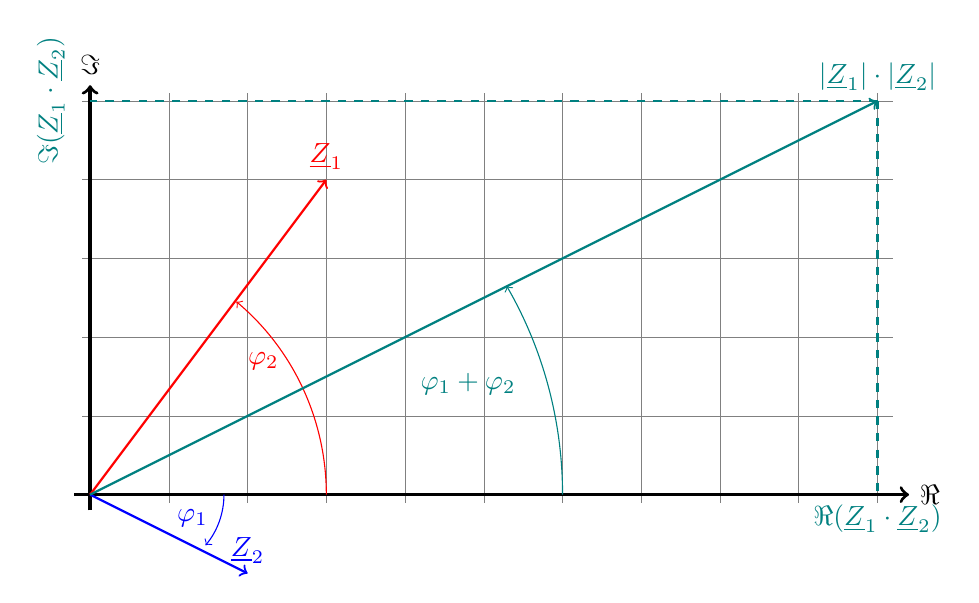
\begin{tikzpicture}
                  \draw (0,0) coordinate (K);
                  \draw[very thin,gray] (-0.1,-0.1) grid (10.2,5.1);
                  \draw[->, very thick] (-0.2,0) -- (10.4,0) node[right] {$\Re$};
                  \draw[->, very thick] (0,-0.2) -- (0,5.2) node[above] {$\Im$};
                  
                  \draw[->, thick, red] (0,0) -- (3,4) node[above] {$\underline{Z}_\mathrm{1}$};
                  \draw[->, thick, blue] (0,0) -- (2,-1) node[above] {$\underline{Z}_\mathrm{2}$};
                  \draw [->,blue] (1.7,0) arc (0:-40:1cm);
                  \draw [->,red] (3,0) arc (0:50:3.2cm);
                  \draw [->,teal] (6,0) arc (0:30:5.3cm);
                  \draw[->, thick, teal] (0,0) -- (10,5) node [above] {$|\underline{Z}_\mathrm{1}| \cdot |\underline{Z}_\mathrm{2}|$};
                  % {{\bf Multiplikation von komplexen Zahlen.} Zeichnerische Lösung einer Multiplikation von zwei komplexen Zahlen im Zeigerdiagramm}
                  \draw[dashed, thick, teal] (10,5) -- (10,0) node[below] {$\Re(\underline{Z}_\mathrm{1} \cdot \underline{Z}_\mathrm{2}$)};
                  \draw[dashed, thick, teal] (10,5) -- (0,5)
                  (-0.5,5) node[rotate=90] {$\Im(\underline{Z}_\mathrm{1} \cdot \underline{Z}_\mathrm{2}$)};
                  \node [red] at (2.2,1.7) {$\varphi_\mathrm{2}$};
                  \node [blue] at (1.3,-0.3) {$\varphi_\mathrm{1}$};
                  
                  \node [teal] at (4.8,1.4) {$\varphi_\mathrm{1} + \varphi_\mathrm{2}$};
              \end{tikzpicture}\\